
\documentclass{beamer}

\usepackage{algpseudocode, color, colortbl, listings, MnSymbol}

\usepackage{hyperref}
\hypersetup{
    colorlinks=true,
    urlcolor=blue,
}

\usetheme{Montpellier}
\usecolortheme{rose}

% page numbers, from
% https://tex.stackexchange.com/questions/137022/how-to-insert-page-number-in-beamer-navigation-symbols
\expandafter\def\expandafter\insertshorttitle\expandafter{%
  \insertshorttitle\hfill%
  \insertframenumber\,/\,\inserttotalframenumber}

\definecolor{Gray}{gray}{0.8}
\newcolumntype{g}{>{\columncolor{Gray}}c}

\newcommand{\stanza}{ \\~\ }

\title{15. Approximate Set Cover and Bin Packing}
\subtitle{CPSC 535}
\author{Kevin A. Wortman}
\institute{ 
\includegraphics[height=2cm]{csuf-logo-cmyk} }
\date{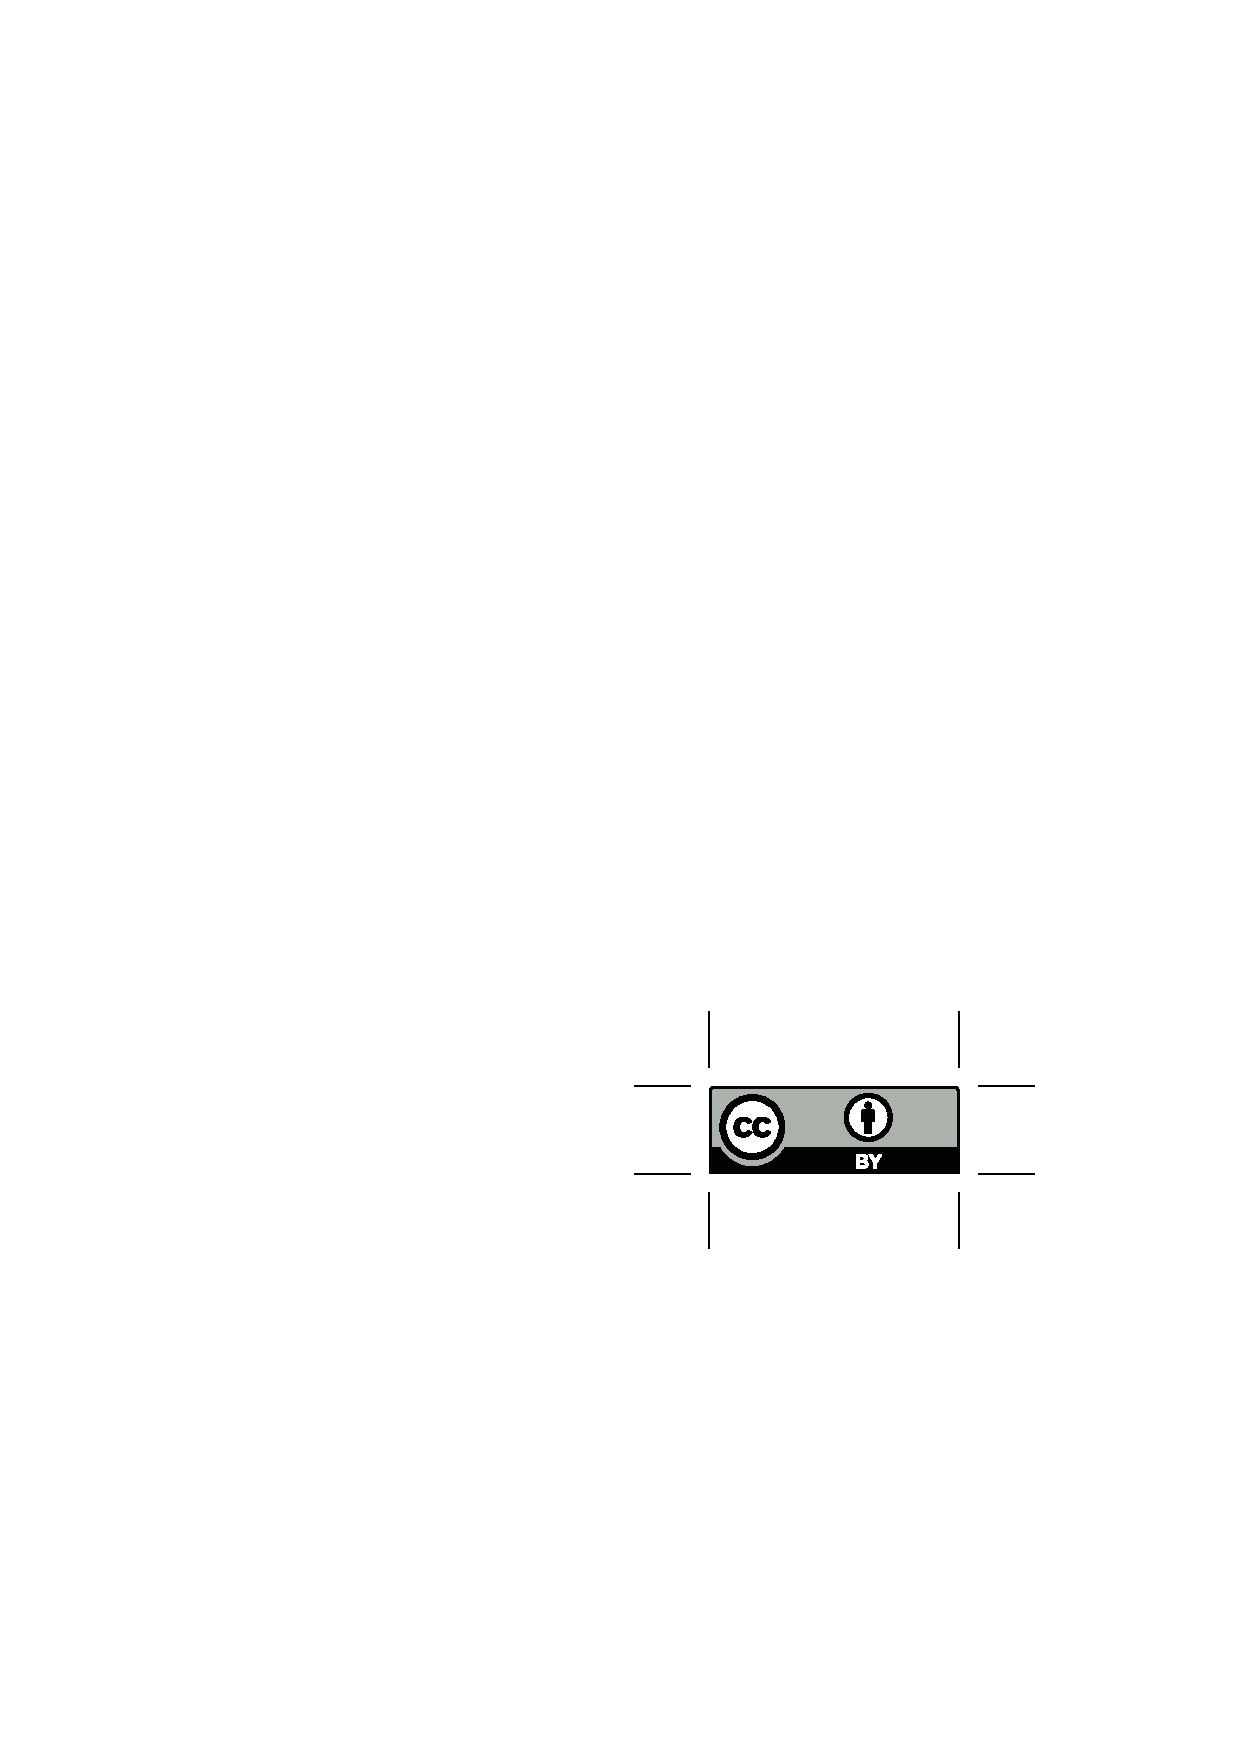
\includegraphics[height=14pt]{by} \\

{\tiny
This work is licensed under a
\href{http://creativecommons.org/licenses/by/4.0/}{Creative Commons Attribution 4.0 International License}.
}}

\begin{document}

\begin{frame}
  \titlepage
\end{frame}

\begin{frame} \frametitle{Set Cover: Intuition}
\end{frame}

\begin{frame} \frametitle{Set Cover: Formal Definition}
\end{frame}

\begin{frame} \frametitle{Set Cover Examples}
\end{frame}

\begin{frame} \frametitle{Set Cover Hardness}
\end{frame}

\begin{frame} \frametitle{Set Cover Approximation Algorithm}
\end{frame}

\begin{frame} \frametitle{Efficiency Analysis}
\end{frame}

\begin{frame} \frametitle{Approximation Ratio}
\end{frame}

\begin{frame} \frametitle{Set Cover Summary}
\end{frame}

\begin{frame} \frametitle{Bin Packing: Intuition}
\end{frame}

\begin{frame} \frametitle{Bin Packing: Formal Definition}
\end{frame}

\begin{frame} \frametitle{Bin Packing Examples}
\end{frame}

\begin{frame} \frametitle{Bin Packing Hardness}
\end{frame}

\begin{frame} \frametitle{Bin Packing Approximation Algorithm}
\end{frame}

\begin{frame} \frametitle{Efficiency Analysis}
\end{frame}

\begin{frame} \frametitle{Approximation Ratio}
\end{frame}

\begin{frame} \frametitle{Bin Packing Summary}
\end{frame}


\end{document}
